\documentclass[11pt]{article}
\usepackage[top=1.00in, bottom=1.0in, left=1.1in, right=1.1in]{geometry}
\renewcommand{\baselinestretch}{1.1}
\usepackage{graphicx}
\usepackage{natbib}
\usepackage{gensymb}
\usepackage{amsmath}
\usepackage{lineno}


\def\labelitemi{--}
\parindent=0pt

\usepackage{Sweave}
\begin{document}
\bibliographystyle{/Users/Lizzie/Documents/EndnoteRelated/Bibtex/styles/besjournals}
\renewcommand{\refname}{\CHead{}}
\begin{flushright}
Version dated: \today
\end{flushright}
\bigskip
\medskip
\begin{center}

\noindent{\Large {\bf Limiting cues: How spring warming, winter chilling and daylength will shape climate change responses}}\\ 
\bigskip

\noindent {\normalsize \sc
The lab as it was in 2017$^{1,2}$}\\ % Ailene, Cat, Dan, Lizzie, Nacho
\noindent {\small \it
$^1$ Arnold Arboretum of Harvard University, 1300 Centre Street, Boston, Massachusetts, 02131, USA\\
$^2$ Organismic \& Evolutionary Biology, Harvard University, 26 Oxford Street, Cambridge, Massachusetts, 02138, USA\\
$^3$ Forest \& Conservation Sciences, Faculty of Forestry, University of British Columbia, 2424 Main Mall, Vancouver, BC V6T 1Z4}\\
\end{center}

\section{Overview of OSPREE}
Studies versus papers ... how many crops versus wild species ....

% Add info on ..
% earliest and latest studies
% types of events
% cleaning is hard, that's why the data are old?
% table of studies

We built the Observed Spring Phenology Responses in Experimental Environments (OSPREE) database, by searching  both ISI Web of Science and Google Scholar  the following terms: 
\begin{enumerate}
\item TOPIC = (budburst OR leaf-out) AND (photoperiod or daylength) AND temperature*, which yielded 85 publications
\item TOPIC = (budburst OR leaf-out) AND dorman*, which yielded 193 publications
\end{enumerate}

\section{Trends in experimental treatments over space}


The actual cues studied varied across latitude with a general trend toward examining more extreme values at higher latitudes. Thus, forcing and chilling treatments decline 0.1$\degree$C per 1 $\degree$ latitude (for forcing, min is -0.1, for max it's -0.06, see Fig \ref{fig:lat}; for chilling it's -0.06 for min and -0.09 for max); and the maximum studied photoperiod increases with latitude (0.09 hr per degree $\degree$ latitude). 


\begin{figure}[t!]
\centering
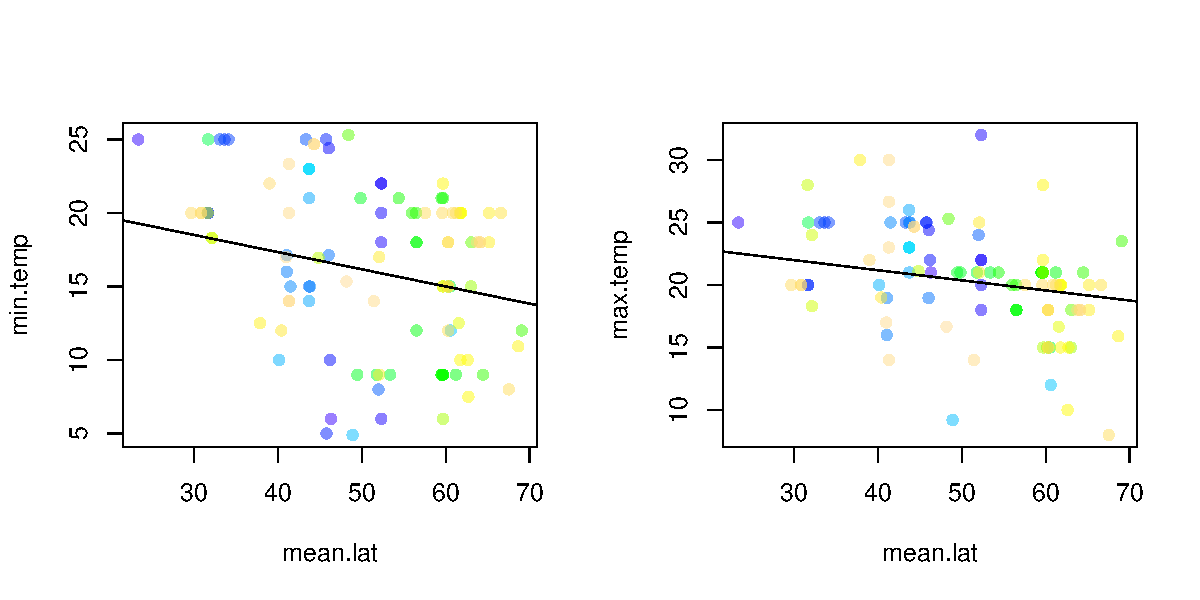
\includegraphics[width=1\textwidth]{..//..//analyses/limitingcues/figures/tempxlatminmaxcorr.pdf}
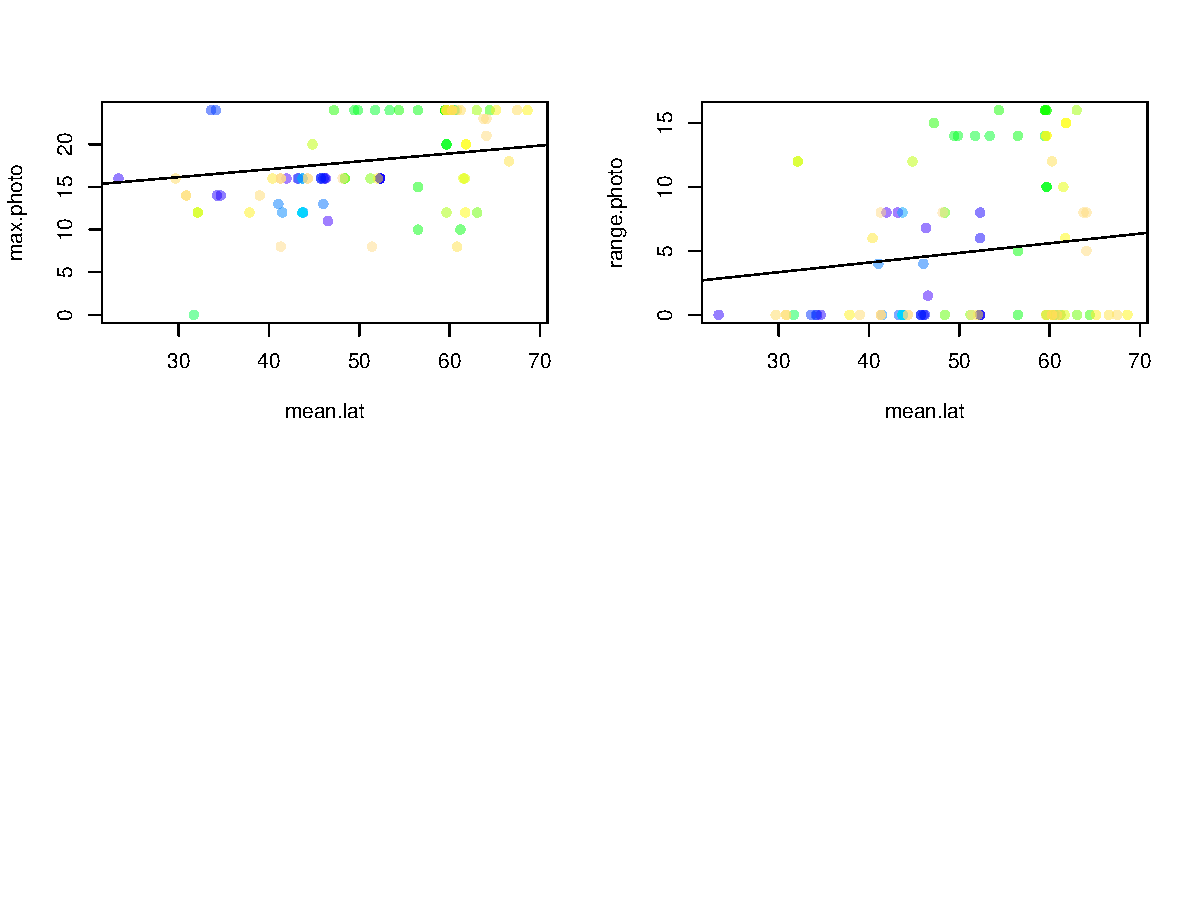
\includegraphics[width=1\textwidth]{..//..//analyses/limitingcues/figures/photoxlatcorr2plots.pdf}
\caption{Some correlations with latitude plots.}
  \label{fig:lat}
\end{figure}


\end{document}





